\documentclass[
    pdflatex,
    fontsize=8pt,
    draft=true,
    twoside
]{article}
\usepackage{emptypage}
\usepackage{watermark}
\usepackage{needspace}
\usepackage{fontawesome5}
\usepackage[utf8]{inputenc}
\usepackage[T1]{fontenc}
\usepackage[
    nohead,
    nomarginpar,
    a5paper,
    bindingoffset=8mm,
    twoside,
    asymmetric,
    % left=6mm,
    % right=6mm,
    % outermargin=12mm,
    width=120mm,
    top=12mm,
    bottom=16mm
]{geometry}
\usepackage{array}
\usepackage{makecell}
\usepackage{qrcode}
\usepackage{hyperref}
\hypersetup{
    colorlinks, linkcolor=black
}
\usepackage{pgfpages}
\usepackage{fancyhdr}
\usepackage[style=iso]{datetime2}
\pagestyle{fancy}
\fancyhead[LE,RO]{}
\fancyhead[LO,RE]{}
\renewcommand{\headrulewidth}{0pt}
\renewcommand{\footrulewidth}{0.2pt}
\usepackage{tabularx}
\usepackage{tabularray}
\setlength{\parindent}{0pt}
\usepackage[english]{babel}
\usepackage{lipsum}
\usepackage{xparse}
\usepackage{multirow}

\NewDocumentCommand{\WineEntry}{ m m m m m m m m m }{
    % Price and wine details row
    #1 / #2 & {#3 #4 #5 \\ #6 \\ #7} & {#8} \\
    % #1 - Glass Price
    % #2 - Bottle Price
    % #3 - Vintage
    % #4 - Winery
    % #5 - Name of Wine
    % #6 - Grape Variety
    % #7 - Winemaker
    % #8 - Region
    % #9 - Description
    % #1 & {#2 #3 \\ #4 \\ #5} & {#6} \\
    % Description row
    \SetCell[c=3]{\linewidth}{#9} \\
    % Spacing row
    \SetCell[c=3]{\linewidth} & & \\
}

\usepackage[absolute,overlay]{textpos}
\usepackage{graphicx}
% \usepackage{txfonts}
\usepackage{marvosym}

%%%%%%%%%%%%%%%%%%%%%%%%%%%%%%%%%%%%%%%%%%%%%%%%%%%%%%%%%%%%%%%%%%%%%%%%
% tabularray: longtblr stuff
%%%%%%%%%%%%%%%%%%%%%%%%%%%%%%%%%%%%%%%%%%%%%%%%%%%%%%%%%%%%%%%%%%%%%%%%
\RenewDocumentCommand\TblrAlignBoth{}{\justifying}
\DefTblrTemplate{contfoot}{default}{}   % Removes text denoting continuation on next page

\NewTblrTheme{TASMenu}{
    \DefTblrTemplate{caption-tag}{default}{}
    \DefTblrTemplate{caption-sep}{default}{}
    % \SetTblrInner{rowsep=2em}
}
\SetTblrOuter[longtblr]{
    postsep=.5\bigskipamount
}
\SetTblrInner[longtblr]{
    belowsep=0pt
}

% \SetTblrInner{abovesep=0pt, belowsep=0pt}



%%%%%%%%%%%%%%%%%%%%%%%%%%%%%%%%%%%%%%%%%%%%%%%%%%%%%%%%%%%%%%%%%%%%%%%%
% Macros
%%%%%%%%%%%%%%%%%%%%%%%%%%%%%%%%%%%%%%%%%%%%%%%%%%%%%%%%%%%%%%%%%%%%%%%%

\newcommand*\TableStart{%
\begin{tabular*}{\linewidth}{@{\extracolsep{\fill} } l l r}
}


\newcommand*\MenuSection[1]{%
    \multicolumn{3}{c}{\LARGE{#1}} \\ \hline \hline \\
}

\newcommand*\TableEnd{%
\end{tabular*}
}

% params:
% 1. Price Big     | 1a
% 2. Price Small   | 1b
% 3. Vintage       | 2
% 4. Winery        |
% 5. Name of Wine  |
% 6. Grape Variety |
% 7. Winemaker     |
% 8. Region        |
\newcommand*\LineItem[8]{
    \makecell[l]{#1 / #2} & \makecell[l]{#3 #4 #5 #6 \\ #7} & \makecell[r]{#8} \\
}

\newcommand*\ItemDescription[1]{%
    \multicolumn{3}{p{\textwidth}}{#1} \\
}

\newcommand*\BlankRow{%
    \multicolumn{3}{c}{ ~ } \\
}

\newcommand*\FoodBlankRow{%
    \multicolumn{3}{c}{ ~ } \\
}

\newcommand*\FoodDescription[1]{%
    \multicolumn{2}{p{120mm}}{\fontsize{8pt}{8pt}{#1}} \\
}

\begin{document}

\begin{centering}
    
\includegraphics[
        width=\textwidth
    ]{Art Syndicate_LOGO_v2_FINAL.png} \\
    % The actual logo goes here. This is just a placeholder.
\end{centering}

\newpage
% 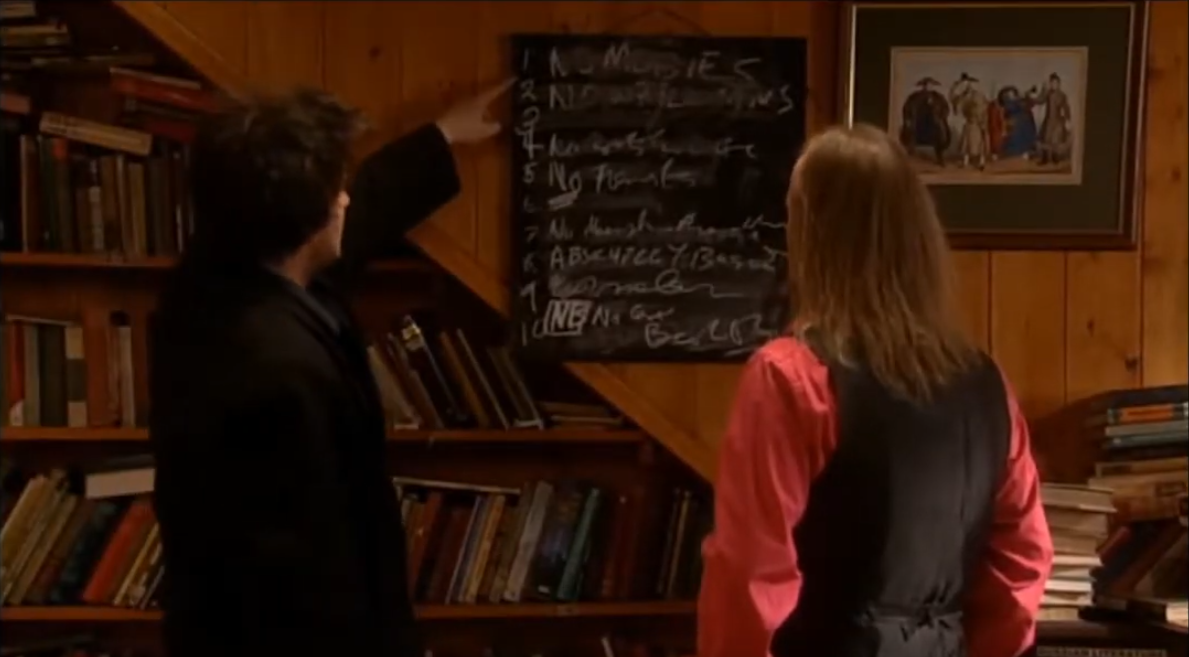
\includegraphics{rules.png}
\begin{tabular}{c m{120mm} c}
    \MenuSection{House Rules}
    \ItemDescription{~}
\end{tabular}

\begin{enumerate}
    \item No name-dropping. Leave your entitlement and status at the door.
    \item Please respect our neighbours' property. Refrain from smoking or loitering outside.
    \item Direct and severe eye contact is recommended for all patrons toasting.
    \item No yelling, hollering, shouting, fighting, screaming, or other loud behaviour unless it is an attempt to warn fellow patrons or employees of impending doom or a police raid.
    \item Feel free to work or play here in a manner consistent with other patrons' peaceful enjoyment.
    \item Do not bring anyone unless you would leave that person alone in your home. You are responsible for the behaviour of your guests. This place is meant to be a home away from home for all patrons; do not be ``that person''.
    \item We are here to serve and tell stories. If you would like to delve deeper into what you are drinking, what adorns the walls, and the history behind such things, feel free to ask questions.
    \item We do not have a superior bathroom for clandestine indulgences. Take the hint, and refrain from bringing such activities into our establishment.
    \item Exit the bar swiftly and quietly. People are endeavouring to sleep across the street and above us. Kindly finalise your travel plans and bid your farewells before departing the premises.
\end{enumerate}
~\\~\\~\\~\\~\\~\\~\\~\\~\\~\\~\\
A surcharge of $10\%$ applies on Sundays and $15\%$ applies on public
holidays.


\newpage
\begin{centering}
    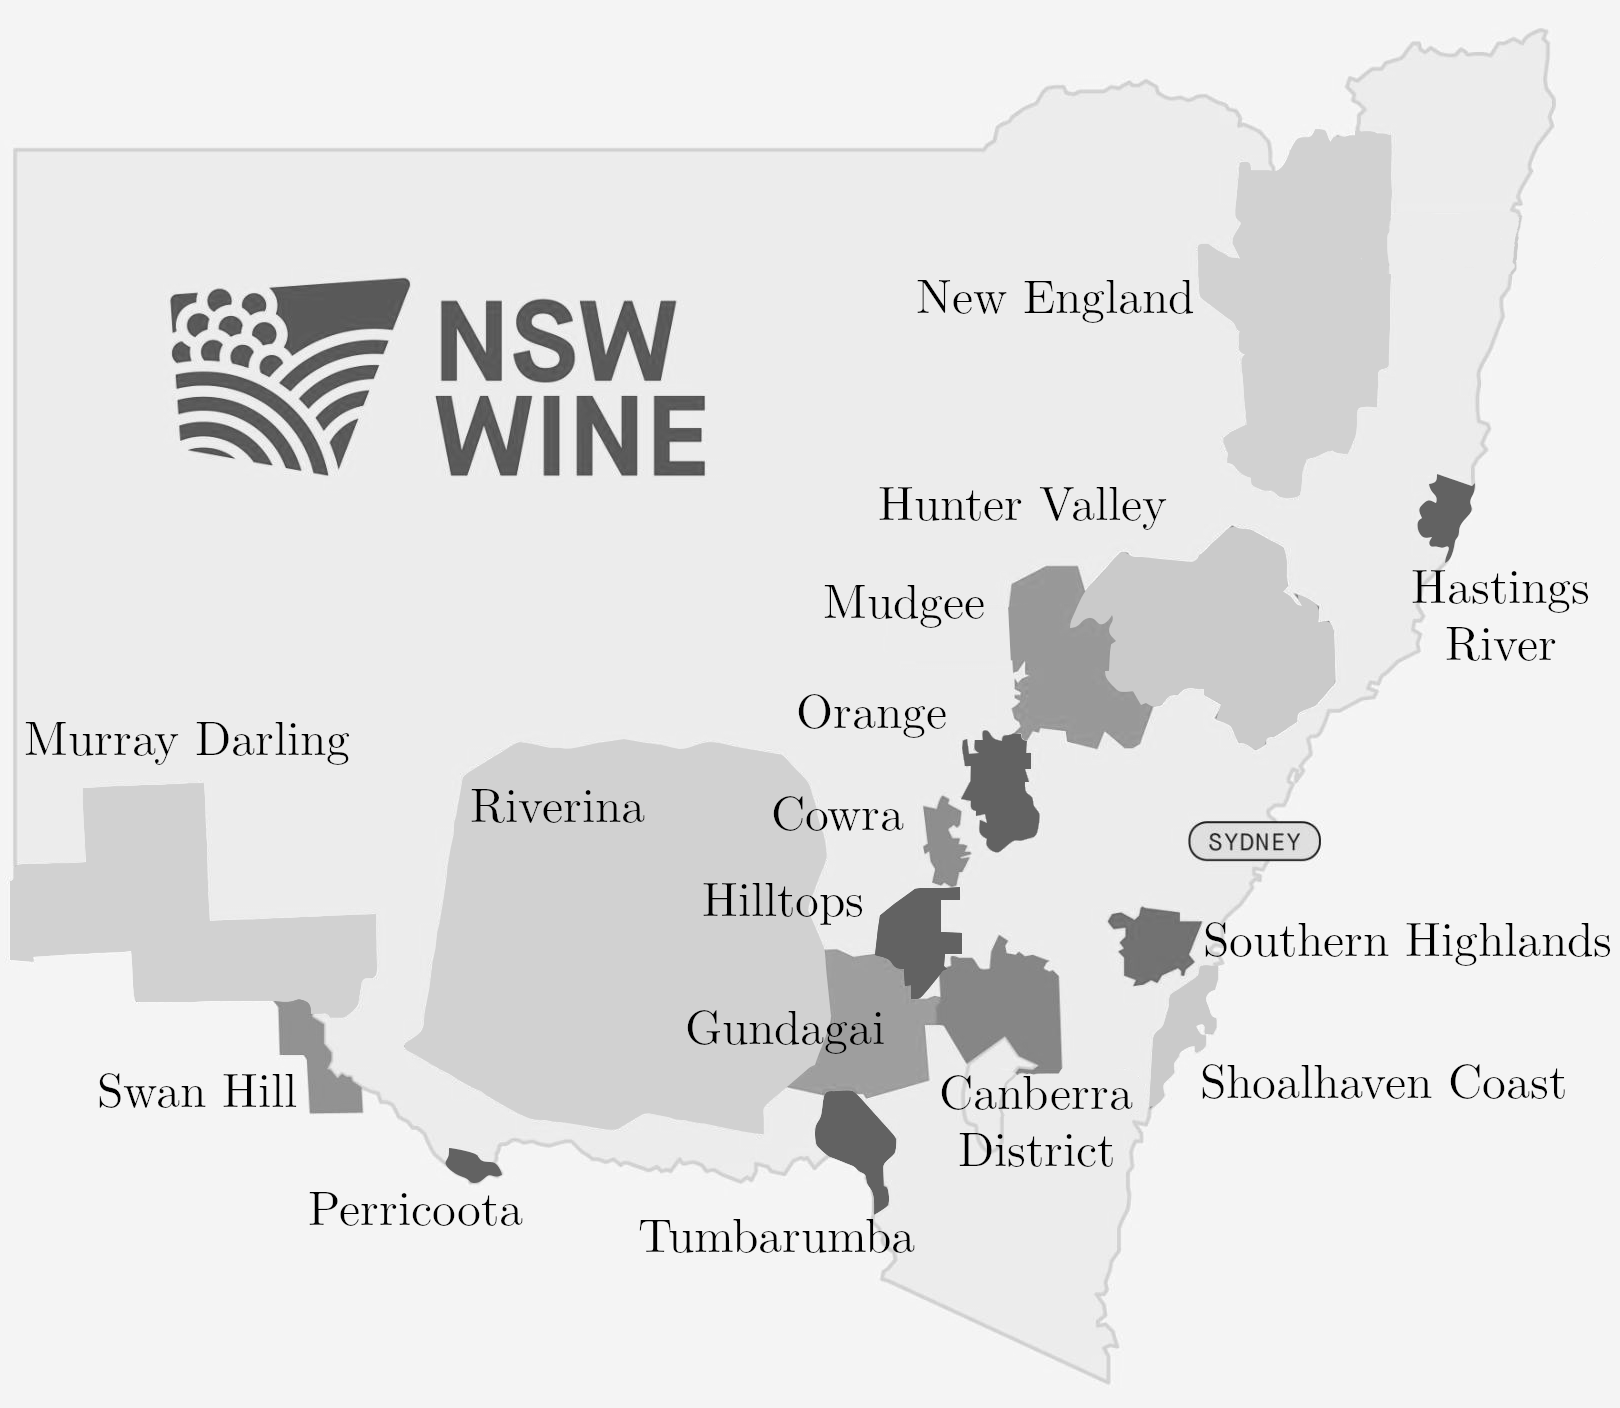
\includegraphics[width=\textwidth]{Wine Map.png}
\end{centering}
\\
At The Art Syndicate, we pride ourselves on exclusively showcasing local wines, beers, and spirits from all over NSW. Each region has unique qualities which manifest themselves in their own distinctive ways. For more information about a region or any of our selection, please do not hesitate to ask Lisa or Saxon!

\newpage

\begin{longtblr}[
    theme = TASMenu,
    caption = \LARGE{Wine - Sparkling},
    halign = j,
    valign = m,
]{
    width = \linewidth,
    colspec = llr,
}

\hline\hline
    \SetCell[c=3]{\linewidth} & & \\
                
    {\\12 / 62} & {NV See Saw Organic Wines "Balance" \\ Prosecco \\ Monica Gray} & {Nashdale, \\Orange Region} \\
    \\
    \SetCell[c=3]{\linewidth}{With over 30 years experience, the family run business is becoming one of Australia's leading organic wine labels. This fresh wine screams lemon sherbet and freshly cut green apple. } \\
    \SetCell[c=3]{\linewidth} & & \\
    
    {\\23 / 130} & {2016 Gallagher Wines "Blanc de Blanc" \\ Chardonnay \\ Greg Gallagher} & {Jeir, \\Canberra District} \\
    \\
    \SetCell[c=3]{\linewidth}{Making wine since the 1970s, Greg’s Blanc de Blanc is a great example of his meticulous approach to winemaking. Made in the “traditional method”, this current vintage was aged for 7 years and developed beautiful aromas of honeydew melon, buttery pastry and a creamy texture.} \\
    \SetCell[c=3]{\linewidth} & & \\
    
    {\\15 / 84} & {2021 Topper's Mountain Wines "Rosé Extra Brut" \\ Nebbiolo \\ Mark and Stephanie Kirkby} & {New England} \\
    \\
    \SetCell[c=3]{\linewidth}{High up above 900m, the ten hectare vineyard specialises in alternative varieties. The Kirkby's don't use any pesticides, but rather promote a balanced ecosystem that is able to help itself. As the only sparkling Nebbiolo made in Australia, it is full of fresh rosehip and wild strawberry aromas with a creamy texture. } \\
    \SetCell[c=3]{\linewidth} & & \\
    
    \end{longtblr}

\vspace{-15pt} 
\pagebreak
\begin{longtblr}[
    theme = TASMenu,
    caption = \LARGE{Wine - White},
    halign = j,
    valign = m,
]{
    width = \linewidth,
    colspec = llr,
}

\hline\hline
    \SetCell[c=3]{\linewidth} & & \\
                
    {\\16 / 76} & {2024 Samantha May Wines  \\ Riesling \\ Samantha Sutherland} & {Orange, \\Mudgee} \\
    \\
    \SetCell[c=3]{\linewidth}{Taking inspiration from her travels and great wines from around the world, Sam focuses on crafting small-batch, single-vineyard wines, to be enjoyed and shared in good company. The wine is full of zesty citrus notes, while gentle oak ageing gives a pleasant texture. } \\
    \SetCell[c=3]{\linewidth} & & \\
    
    {\\15 / 72} & {2024 Mada Wines "Blanc" \\ Pinot Gris, Gtramz, Riesling \\ Hamish Young} & {Hilltops} \\
    \\
    \SetCell[c=3]{\linewidth}{Dedicated to showcasing the potential of the Canberra, Hilltops, and Tumbarumba regions, Hamish collaborates with viticulturalists who share his philosophy. This is a generous blend, with aromas of orange blossom, fresh lychee and lots of zestiness. } \\
    \SetCell[c=3]{\linewidth} & & \\
    
    {\\14 / 67} & {2023 Tumblong Hills  \\ Chenin Blanc \\ Simon Robertson} & {Gundagai} \\
    \\
    \SetCell[c=3]{\linewidth}{Tumblong Hills' philosophy is all about thoughtful vineyard practices, respecting nature and working to protect the environment. Chenin Blanc is originally from France but has found perfect growing conditions in NSW with classic notes of honeysuckle, pear and quince.} \\
    \SetCell[c=3]{\linewidth} & & \\
    \pagebreak
    \\    
    {\\18 / 87} & {2021 Wondalma Vineyard  \\ Chardonnay \\ Stuart and Janine Barclay} & {Tumbarumba} \\
    \\
    \SetCell[c=3]{\linewidth}{Renowned for growing outstanding Chardonnay in Tumbarumba, this wine is from their own label. Fresh flavours of white peaches and grapefruit are complemented by creamy and flinty notes from gentle oak ageing. } \\
    \SetCell[c=3]{\linewidth} & & \\
    
    {\\25 / 120} & {2023 Origines "Focus" \\ Chardonnay \\ Alex Beckett and Jan Taborsky} & {Orange} \\
    \\
    \SetCell[c=3]{\linewidth}{Meeting in the Master of Wine program, the winemakers connected over their passion for small-batch, terroir driven wine. The thoughtful approach to winemaking and long oak maturation created a layered, ever evolving wine with aromas of lemon curd, fresh yellow apple and baking spices.} \\
    \SetCell[c=3]{\linewidth} & & \\
    
    {\\18 / 87} & {2024 Matthew Attalah Wines "Block 5, La Femme Nikita" \\ Sauvignon Blanc \\ Matthew Attalah} & {Orange} \\
    \\
    \SetCell[c=3]{\linewidth}{Wth a focus on texture, finesse and balance in all his wines, Matt believes that wines from Orange can stand proudly alongside the world’s best. Taking inspiration from styles of the french Loire Valley, the wine is laden with tropical fruits and herbaceous texture from the extended time in older oak barrels.} \\
    \SetCell[c=3]{\linewidth} & & \\
    
    {\\27 / 130} & {2014 Silkman Wines "Blackberry" \\ Semillon \\ Liz Silkman} & {Pokolbin, \\Hunter Valley} \\
    \\
    \SetCell[c=3]{\linewidth}{Being named Halliday Winemaker of the Year 2025, Liz’s vision is to make some of the best small batch contemporary versions of traditional Hunter varieties. This aged Semillon shows intense flavours of preserved lemon, chamomile and mouthcoating notes of crème brulee and green almonds.} \\
    \SetCell[c=3]{\linewidth} & & \\
    
    \end{longtblr}

\vspace{-15pt} 
\pagebreak
\begin{longtblr}[
    theme = TASMenu,
    caption = \LARGE{Wine - Amber},
    halign = j,
    valign = m,
]{
    width = \linewidth,
    colspec = llr,
}

\hline\hline
    \SetCell[c=3]{\linewidth} & & \\
                
    {\\17 / 84} & {2021 Topper's Mountain Wines "Hill of Dreams" \\ Sauvignon Blanc, Verdejo, \\
Grüner Veltliner \\ Mark and Stephanie Kirkby} & {New England} \\
    \\
    \SetCell[c=3]{\linewidth}{High up above 900m, the ten hectare vineyard specialises in alternative varieties. The Hill of Dreams is a place of diversity and experimentation. The different varieties are spontaneously fermented on their skins for texture and fragrant notes of jalapeno, preserved lemon and gooseberry compote.  } \\
    \SetCell[c=3]{\linewidth} & & \\
\end{longtblr}

\vspace{-15pt} 

\begin{longtblr}[
    theme = TASMenu,
    caption = \LARGE{Wine - Rosé},
    halign = j,
    valign = m,
]{
    width = \linewidth,
    colspec = llr,
}

\hline\hline
    \SetCell[c=3]{\linewidth} & & \\
                
    {\\14 / 67} & {2023 Sapling Yard "The Four Pinots" \\ Gris, Noir, Meunier, Blanc \\ Carla Rodeghiero} & {Tumbarumba and \\ Braidwood} \\
    \\
    \SetCell[c=3]{\linewidth}{Sapling Yard was founded in 2008 when Carla planted her own vineyard in Braidwood at 650 metres above sea level. The blend of Pinots makes an intriguing wine full of depth and flavours of pink grapefruit, raspberry coulis and red apple skin. } \\
    \SetCell[c=3]{\linewidth} & & \\
    \pagebreak
    \\    
    {\\17 / 85} & {2022 Nashdale Lane "Legacy Rosé" \\ Shiraz \\ 	Tanya and Nick Segger} & {Nashdale, \\Orange} \\
    \\
    \SetCell[c=3]{\linewidth}{The Legacy series is all about a patient winemaking approach. Using the heavier grape pressings and aged in seasoned oak for 10 months, this richer style is for everyone enjoying a chilled red. This wine shows aromas of wild strawberries, raspberries and exotic spices leading to a smooth textured finish.} \\
    \SetCell[c=3]{\linewidth} & & \\
\end{longtblr}

\vspace{-15pt} 

\begin{longtblr}[
    theme = TASMenu,
    caption = \LARGE{Wine - Red},
    halign = j,
    valign = m,
]{
    width = \linewidth,
    colspec = llr,
}

\hline\hline
    \SetCell[c=3]{\linewidth} & & \\
                
    {\\15 / 78} & {2023 Renzaglia Wines "Nuovo di Renzo" \\ Sangiovese, Graciano, Merlot, Shiraz, \\
Cabernet Sauvignon \\ Sam Renzaglia } & {O'Connell Valley, \\Central Ranges} \\
    \\
    \SetCell[c=3]{\linewidth}{The Renzaglia family sees themselves as `Stewards of the vines' with a balanced ecosystem in mind. Their "di Renzo" label explores unique styles through innovative and creative winemaking techniques. This chilled red is full of fresh, crunchy fruit and savoury herbaceousness.} \\
    \SetCell[c=3]{\linewidth} & & \\
    
    {\\17 / 83} & {2023 Sabi Wabi "Nomu" \\ Syrah \\ Peta Kotz} & {Hunter Valley} \\
    \\
    \SetCell[c=3]{\linewidth}{Peta, a Young Gun Of Wine 2022 - Winemaker's Choice winner, is producing small batch, low-intervention wines. The "Nomu" was made entirely in stainless steel, preserving the fresh fruit flavours and delicate aromas in this lighter style. } \\
    \SetCell[c=3]{\linewidth} & & \\
    \pagebreak
    \\    
    {\\18 / 90} & {2022 Rowlee Wines "Single Vineyard" \\ Pinot Noir \\ Nicole Samodol and James Manny} & {Nashdale, \\Orange} \\
    \\
    \SetCell[c=3]{\linewidth}{Handpicking from an eight-hectare vineyard situated on Orange's ancient volcanic soils, the team at Rowlee focus on small batch winemaking with sustainable practices. Layers of crunchy red fruit with notes of cinnamon and liquorice add to the complexity and depth of the wine.
} \\
    \SetCell[c=3]{\linewidth} & & \\
    
    {\\14 / 65} & {2022 Whitton Farm "Rosso" \\ Sangiovese, Shiraz \\ Caleb Wearne} & {Hilltops, \\Canberra} \\
    \\
    \SetCell[c=3]{\linewidth}{Whitton Farm, driven by a passion for fine Italian wines, produces small-batch handcrafted wines from New South Wales' premium, often overlooked wine regions that share a similar climate to central Italy. The Rosso is a medium bodied blend, boasting red cherries and soft spices. } \\
    \SetCell[c=3]{\linewidth} & & \\
    
    {\\15 / 70} & {2019 The Little Wine Company  \\ Barbera \\ Suzanne and Ian Little} & {Broke, \\Hunter Valley} \\
    \\
    \SetCell[c=3]{\linewidth}{Suzanne and Ian, both from winemaking backgrounds, joined forces in 2000. Originally from Italy’s northern Piedmont region, this Barbera enjoys the Hunter's long sunshine hours and displays plush red and black berries, and soft tannins. } \\
    \SetCell[c=3]{\linewidth} & & \\
    
    {\\18 / 85} & {2018 Glenguin "Aristea" \\ Shiraz \\ Robin, Rita and Andrew Tedder} & {Hunter Valley} \\
    \\
    \SetCell[c=3]{\linewidth}{Under the guidance of Master of Wine Robin Tedder, the estate follows organic and biodynamic principles to produce limited, high-quality Shiraz and Semillon from vines descended from James Busby’s original 1820s plantings. Powerful yet refined, the wine has notes of ripe berries, dark chocolate and Christmas cake. } \\
    \SetCell[c=3]{\linewidth} & & \\
    \pagebreak
    \\    
    {\\14 / 69} & {2015 Quilty Wines "Silken Thread" \\ Petit Verdot \\ Des Quilty} & {Mudgee} \\
    \\
    \SetCell[c=3]{\linewidth}{Des Quilty, known for making age worthy, single parcel reds, has been working as a viticulturist for 20 years. The wine is from a tiny plot of hand-picked grapes from low-yielding vines on the Southern edge of Mudgee, with only 178 cases produced. This beautifully aged wine has developed intense aromas of vanilla bean, macerated blueberries and forest fruits. } \\
    \SetCell[c=3]{\linewidth} & & \\
\end{longtblr}

\vspace{-15pt} 

\begin{longtblr}[
    theme = TASMenu,
    caption = \LARGE{Wine - Sweet},
    halign = j,
    valign = m,
]{
    width = \linewidth,
    colspec = llr,
}

\hline\hline
    \SetCell[c=3]{\linewidth} & & \\
                
    {\\8 / 60} & {2022 Vinifera Wines "Easter" \\ Semillon \\ Sam McKendry} & {Mudgee} \\
    \\
    \SetCell[c=3]{\linewidth}{The McKendry family has been growing grapes organically since 2008, becoming certified organic in 2013. Made from botrytis grapes, the wine shows aromas of honeysuckle while flavours of candied cashews, honey and orange marmalade coat the palate.} \\
    \SetCell[c=3]{\linewidth} & & \\
\end{longtblr}

\vspace{-15pt} 

\begin{longtblr}[
    theme = TASMenu,
    caption = \LARGE{Wine - Non-alcoholic},
    halign = j,
    valign = m,
]{
    width = \linewidth,
    colspec = llr,
}

\hline\hline
    \SetCell[c=3]{\linewidth} & & \\
                
    {\\12 / 55} & {NV Altina "Finger Lime" \\ Sauvignon Blanc \\ Christina Delay and Alan Tse Ca} & {Mitchell, \\Canberra District} \\
    \\
    \SetCell[c=3]{\linewidth}{In 2018, Christina and Alan went on a mission to craft complex drinks combining premium Australian wine with botanicals. Their de-alcoholised Sauvignon Blanc features aromas of white nectarine, fresh cucumber, and notes of pepper and lemon grass.} \\
    \SetCell[c=3]{\linewidth} & & \\
    
    \end{longtblr}

\vspace{-15pt} 
\pagebreak

%\newpage
% \begin{longtblr}[
%     theme = TASMenu,
%     caption = \LARGE{Tap Beer},
%     halign = j,
%     valign = m,
% ]{
%     width = \textwidth,
%     colspec = cll,
%     % hlines,
%     % vlines,
% }
% \hline\hline
% \SetCell[c=3]{\linewidth} & & \\
% 9.5 & {Tap beer \\ } &                             Ask about our latest tap beers, or just look at our tap. \\
% \end{longtblr}

% \newpage

\begin{longtblr}[
    theme = TASMenu,
    caption = \LARGE{Beer \& Cider},
    halign = j,
    valign = m,
]{
    width = \textwidth,
    colspec = cll,
    % hlines,
    % vlines,
}
\hline\hline

\SetCell[c=3]{\linewidth} & & \\
9 & { \\ } & Sydney Tap Beer \\

\SetCell[c=3]{\linewidth} & & \\
13 & {Willie the Boatman \\ St Peters, Sydney} & 'Rogue'' Lager \\

\SetCell[c=3]{\linewidth} & & \\
13 & {Willie the Boatman \\ St Peters, Sydney} & 'Andy Smash'' Hazy Pale Ale  \\

\SetCell[c=3]{\linewidth} & & \\
13 & {Yulli's Brews \\ Alexandria, Sydney} & 'Dolly Aldrin'' Yuzu Berliner Weisse \\

\SetCell[c=3]{\linewidth} & & \\
12 & {Yulli's Brews \\ Alexandria, Sydney} & 'Margot'' Dry Apple Cider \\

\SetCell[c=3]{\linewidth} & & \\
15 & {Powder Monkey Brewing Co. \\ St Peters, Sydney} & Cherry Sour \\

\SetCell[c=3]{\linewidth} & & \\
13 & {Willie the Boatman \\ St Peters, Sydney} & Alcoholic Ginger Beer \\

\SetCell[c=3]{\linewidth} & & \\
10 & {Heaps Normal \\ Marrickville, Sydney} & 'Quiet'' XPA \\

\end{longtblr}


\newpage

\begin{longtblr}[
    theme = TASMenu,
    caption = \LARGE{Cocktails},
    halign = j,
    valign = m,
]{
    width = \linewidth,
    colspec = cll,
    % hlines,
    % vlines,
}
\hline\hline
    \SetCell[c=3]{\linewidth} & & \\

    22 & Negroni & Prefer whisky? Ask about a Boulevardier! \\
    \SetCell[c=3]{\linewidth} & & \\

    23 & Old Fashioned & Made with Brix Distillers Australian rum. \\
    \SetCell[c=3]{\linewidth} & & \\

    22 & Martini & As you like it. \\
    \SetCell[c=3]{\linewidth} & & \\

    19 & Americano &  \\
    \SetCell[c=3]{\linewidth} & & \\

    20 & French 75 &  \\
    \SetCell[c=3]{\linewidth} & & \\

    10 & Vermouth Spritz & Red or white. \\
    \SetCell[c=3]{\linewidth} & & \\

    24 & Pisco Sour &  \\
    \SetCell[c=3]{\linewidth} & & \\

    22 & Passionfruit Spritz &  \\
    \SetCell[c=3]{\linewidth} & & \\

    12 & Hibiscus Spritz & non-alcoholic \\
    \SetCell[c=3]{\linewidth} & & \\

    10 & G\&T with housemade tonic & non-alcoholic \\
    \SetCell[c=3]{\linewidth} & & \\

    12 & Margarita & non-alcoholic \\
    \SetCell[c=3]{\linewidth} & & \\

\end{longtblr}


\newpage

\begin{longtblr}[
    theme = TASMenu,
    caption = \LARGE{Spirits - Gin},
    halign = j,
    valign = m,
]{
    width = \linewidth,
    colspec = cll,
    % hlines,
    % vlines,
}
\hline\hline
    \SetCell[c=3]{\linewidth} & & \\

    10 & {The Primary Goods Co. Distillery \\ Parramatta} & {Section 72 Gin} \\
    \SetCell[c=3]{\linewidth} & & \\

    13 & {Hickson House Distilling Co. \\ The Rocks, Sydney} & {Seven Spice } \\
    \SetCell[c=3]{\linewidth} & & \\

    13 & {} & {Australian Dry Gin } \\
    \SetCell[c=3]{\linewidth} & & \\

    14 & {} & {Oyster Shell Gin } \\
    \SetCell[c=3]{\linewidth} & & \\

    16 & {Joadja Distillery \\ Joadja} & {Barrel Aged Gin} \\
    \SetCell[c=3]{\linewidth} & & \\

\end{longtblr}


\begin{longtblr}[
    theme = TASMenu,
    caption = \LARGE{Spirits - Vodka},
    halign = j,
    valign = m,
]{
    width = \linewidth,
    colspec = cll,
    % hlines,
    % vlines,
}
\hline\hline
    \SetCell[c=3]{\linewidth} & & \\

    10 & {Jance Distillery \\ Rouse Hill} & {Rice Vodka} \\
    \SetCell[c=3]{\linewidth} & & \\

    10.5 & {Mobius Distilling Co. \\ Marrickville, Sydney} & {38 Special Vodka} \\
    \SetCell[c=3]{\linewidth} & & \\

    11 & {Scylla Distilling Co. \\ Taren Point, Sydney} & {Vodka} \\
    \SetCell[c=3]{\linewidth} & & \\

\end{longtblr}


\begin{longtblr}[
    theme = TASMenu,
    caption = \LARGE{Spirits - Whisky},
    halign = j,
    valign = m,
]{
    width = \linewidth,
    colspec = cll,
    % hlines,
    % vlines,
}
\hline\hline
    \SetCell[c=3]{\linewidth} & & \\

    12 & {Manly Spirits Co. \\ Manly, Sydney} & {Coastal Stone Xplore Blended Whisky} \\
    \SetCell[c=3]{\linewidth} & & \\

    20 & {Joadja Distillery \\ Joadja} & {Single Malt Whisky Ex Oloroso Sherry Barrel} \\
    \SetCell[c=3]{\linewidth} & & \\

    25 & {} & {Single Malt Whisky Ex Amontillado Sherry Barrel} \\
    \SetCell[c=3]{\linewidth} & & \\

    20 & {} & {Single Malt Whisky, Ex Pedro Ximenez Casks } \\
    \SetCell[c=3]{\linewidth} & & \\

    15 & {Corowa Distilling Co.  \\ Corowa} & {The Ben Buckler} \\
    \SetCell[c=3]{\linewidth} & & \\

    18 & {} & {Corowa Characters} \\
    \SetCell[c=3]{\linewidth} & & \\

    25 & {} & {Bosque Verde} \\
    \SetCell[c=3]{\linewidth} & & \\

    20 & {} & {Barrel House XB Peated} \\
    \SetCell[c=3]{\linewidth} & & \\

\end{longtblr}


\begin{longtblr}[
    theme = TASMenu,
    caption = \LARGE{Spirits - Rum},
    halign = j,
    valign = m,
]{
    width = \linewidth,
    colspec = cll,
    % hlines,
    % vlines,
}
\hline\hline
    \SetCell[c=3]{\linewidth} & & \\

    13 & {Brix Distillers \\ Surry Hills, Sydney} & {Australian Rum} \\
    \SetCell[c=3]{\linewidth} & & \\

    12 & {} & {Citrus Got Real Mandarin Liqueur} \\
    \SetCell[c=3]{\linewidth} & & \\

\end{longtblr}


\begin{longtblr}[
    theme = TASMenu,
    caption = \LARGE{Spirits - Liqueur},
    halign = j,
    valign = m,
]{
    width = \linewidth,
    colspec = cll,
    % hlines,
    % vlines,
}
\hline\hline
    \SetCell[c=3]{\linewidth} & & \\

    10 & {Jance Distillery \\ Rouse Hill} & {Honey Liqueur} \\
    \SetCell[c=3]{\linewidth} & & \\

    11 & {Scylla Distilling Co. \\ Taren Point, Sydney} & {Raspberry Liqueur} \\
    \SetCell[c=3]{\linewidth} & & \\

    11 & {} & {Passionfruit Liqueur} \\
    \SetCell[c=3]{\linewidth} & & \\

\end{longtblr}




\begin{longtblr}[
    theme = TASMenu,
    caption = \LARGE{More Spirits from NSW},
    halign = j,
    valign = m,
]{
    width = \linewidth,
    colspec = cll,
    % hlines,
    % vlines,
}
\hline\hline
    \SetCell[c=3]{\linewidth} & & \\


    13 & {The Primary Goods Co. Distillery \\ Parramatta} & { Pisco-esque} \\
    \SetCell[c=3]{\linewidth} & & \\

    13 & {Hoju \\ NSW} & {Soju} \\
    \SetCell[c=3]{\linewidth} & & \\

    12 & {Poor Toms \\ Marrickville, Sydney} & {Imbroglio Amaro} \\
    \SetCell[c=3]{\linewidth} & & \\

    8 & {Regal Rogue  \\ Orange} & {Bold Red Sweet Vermouth} \\
    \SetCell[c=3]{\linewidth} & & \\

    9 & {Joadja Distillery \\ Joadja} & {Sweet Vermouth} \\
    \SetCell[c=3]{\linewidth} & & \\

    9 & {Regal Rogue  \\ Orange} & {Dry Vermouth} \\
    \SetCell[c=3]{\linewidth} & & \\

    7 & {Joadja Distillery \\ Joadja} & {Pedro Ximenez} \\
    \SetCell[c=3]{\linewidth} & & \\

\end{longtblr}


\newpage

\begin{longtblr}[
    theme = TASMenu,
    caption = \LARGE{Non-alcoholic},
    halign = j,
    valign = m,
]{
    width = \linewidth,
    colspec = cll,
    % hlines,
    % vlines,
}
\hline\hline\\

    12 & {"Finger Lime" \\ Mitchell, Canberra District} & Sauvignon Blanc \\
    \SetCell[c=3]{\linewidth} & & \\

    6 & {Sammy Piquant \\ Seven Hills, Sydney} & The Jetsetter Aperitif \\
    \SetCell[c=3]{\linewidth} & & \\

    6 & {Sammy Piquant \\ Seven Hills, Sydney} & The Oaxacan Mezcal \\
    \SetCell[c=3]{\linewidth} & & \\

    7 & {ALTD Spirits \\ Marrickville, Sydney} & Silver Princess Gin \\
    \SetCell[c=3]{\linewidth} & & \\

    9.5 & {Yes You Can \\ Bondi, Sydney} & Yuzu Sake lemonade \\
    \SetCell[c=3]{\linewidth} & & \\

    9.5 & {Sammy Piquant \\ Seven Hills, Sydney} & South Pacific Seltzer \\
    \SetCell[c=3]{\linewidth} & & \\

    9.5 & {Chapter Tea  \\ NSW} & Strawberry \& Basil Ice Tea \\
    \SetCell[c=3]{\linewidth} & & \\

    7 & {Mate} & house made sparkling ice tea \\
    \SetCell[c=3]{\linewidth} & & \\

    6 & {Selection of T2 teas } & ~ \\
    \SetCell[c=3]{\linewidth} & & \\

    4 & {Coffee: Espresso/Long Black} & ~ \\
    \SetCell[c=3]{\linewidth} & & \\

    4.5 & Sparkling water & Unlimited refills \\
    \SetCell[c=3]{\linewidth} & & \\

    -   & {tap\textsuperscript{\texttrademark} by Sydney Water \\ Wollondilly Shire } & ~ \\
    \SetCell[c=3]{\linewidth, halign=l} Bearing no notes or hints of anything, this special blend suits all tastes. Officially known as ``tap\textsuperscript{\texttrademark} A Sydney Water Product'', locals refer to it as the ``Warragamba Slammer'' & ~ & ~ \\
    
\end{longtblr}


\newpage

\begin{longtblr}[
    theme = TASMenu,
    caption = \LARGE{Food},
    halign = j,
    valign = m,
]{
    width = \linewidth,
    colspec = cll,
    % hlines,
    % vlines,
}
\hline\hline

    5 & Olives & { Parafield Olives "Wallis", Yarragundry, NSW} \\
    \SetCell[c=3]{\linewidth} & & \\

    12.5 & Toastie & {Cheese, butter, house made kimchi jam.} \\
    \SetCell[c=3]{\linewidth} & & \\

    5.5 & Soya Chips & {Irresistibly snackable.} \\
    \SetCell[c=3]{\linewidth} & & \\

    8 & Snickerdoodle Cookie & {House made by Saxon.} \\
    \SetCell[c=3]{\linewidth} & & \\

\end{longtblr}

Please be aware that our dishes may contain allergens such as nuts,
seafood, gluten, soy, eggs, and dairy.

\newpage
At The Art Syndicate, we offer a unique experience by immersing guests in a collection of original vintage posters and contemporary art spanning from the late 1800s through to present day. We create an engaging atmosphere that seamlessly combines historical appreciation with contemporary style. For those with a interest in building their own collection, we welcome you to arrange a private appointment to explore our stockroom. Alternatively, you can conveniently browse and acquire original artworks through our website. Whether you're seeking a distinctive addition to your establishment or a meaningful acquisition for your personal collection, The Art Syndicate can find the perfect artwork for you.
\\~\\
\begin{center}
    \qrcode{https://www.theartsyndicate.com.au}
    \\~\\
    \url{www.theartsyndicate.com.au}
\end{center}
\fancyfoot[R]{\footnotesize\DTMnow}
\begin{textblock*}{\linewidth}[0,0](8mm,\dimexpr\paperheight-20mm\relax)
    \footnotesize{
        \texttt{Typeset with $\heartsuit$ in \LaTeX~ by Adam Carmichael in Sydney, NSW}
    }\\
    \footnotesize{
        \texttt{Automated with \faIcon{beer} and \faIcon{python} by Michael Tulskikh in Sydney, NSW}
    }
\end{textblock*}


\end{document}